We now introduce another approach based on the Edgeworth series to create accurate density approximations that avoids some of the issues of the Edgeworth series that we have demonstrated in the previous section.

We now introduce the idea of \textit{exponential tilting}. Consider a random random variable $X \sim \Rp$ with cumulant generative function $K$ and density $f$. We introduce the exponential family $\mathcal{T}_P = \{ P_\gamma \}_{\gamma \in \Rp}$ where each $P_\gamma \in \mathcal{T}_P$ is characterized by its density function $f_\gamma$ given by
\begin{equation*}
    f_\gamma(x) = f(x)\expf{\gamma^\top x - K(\gamma)}.
\end{equation*}
Note that by the definition of the cumulant generating function, $K(\gamma)$ is the right normalization factor for $f_\gamma$ and hence $f_\gamma$ integrates to 1 and is a valid density function. Furthermore, the original distribution $P$ is an element of $\mathcal{T}_P$ with $P = P_0$. Given two distributions in $\mathcal{T}_P$, their densities only differ by the ratio of $\expf{\gamma^\top x - K(\gamma)}$. Since the following holds for any $\gamma \in \Rp$
\begin{equation} \label{eq-saddlepoint-original}
    f(x) = f_\gamma(x)\expf{K(\gamma) - \gamma^\top x},
\end{equation}
we can construct an approximation of $f$ by choosing $\gamma$ such that $f_\gamma$ can be accurately approximated.

Let us now consider a distribution $P$ with cumulant generating function $K$. We wish to use the previous argumentation to approximate the density $f$ of the mean $S$ of $n$ i.i.d.\,random variables distributed according to $P$. The cumulant generating function of $S$ in Equation (\ref{eq-saddlepoint-original}), we get
\begin{equation*}
    f(s) = f_\gamma(s)\expf{nK(\gamma / n) - \gamma^\top s}.
\end{equation*}
We can now get back to the question of the choice of $\gamma$. We are interested in choosing $\gamma$ such that the Edgeworth approximation of $\bar f_\gamma(x)$ is accurate. As seen in Remark \ref{rem-edge-mean}, the second order Edgeworth approximation of odd order gains half an order of accuracy when evaluated at the mean of the distribution. Since $\gamma$ can be chosen freely and differently for each value $s$ at which the density $f(s)$ is evaluated, we can choose $\gamma$ such that $s$ is the mean of the distribution $P_\gamma$. Given $\gamma \in \Rp$, the cumulant generating function of $P_\gamma$ is equal to
\begin{equation*}
    K_\gamma(t) = n\left[K((\gamma + t)/n) - K(\gamma/n)\right].
\end{equation*}
One sees that derivatives of the cumulant generating function $K_\gamma$ can be expressed in terms of the cumulant generating function $K$ by
\begin{equation} \label{eq-deriv-Kgamma}
    K_\gamma^s(t) = n^{1 - k} K((\gamma + t) / n),
\end{equation}
for any $s \in S(k)$. Thus, using a well-known property of exponential families, the expectated value of the distribution $P_\gamma$ can be expressed in terms of the gradient of the cumulant generating function of $X$,
\begin{equation*}
    \expec{S \sim P_\gamma}{S} = K'(\gamma / n).
\end{equation*}
For any $s \in \Rp$, we can now find a distribution $P_{\hat\gamma_s} \in \mathcal{T}_P$ with mean $s$ by solving
\begin{equation} \label{eq-saddlepoint}
    K'(\hat\gamma_s / n) = s.
\end{equation}
We choose to call the solution of this equation $\hat\gamma_s$ to emphasize the fact that instead of choosing one unique $\gamma$ and then construct an approximation of the density of $P_\gamma$ over $\Rp$, we find a different $\hat\gamma_s$ at each $s \in \Rp$ such that the Edgeworth approximation of the density of $P_{\hat\gamma_s}$ is accurate in $s$. Note that if $\hat\gamma_s$ solves (\ref{eq-saddlepoint}), it is also the maximum likelihood estimator of $\gamma$ within the model $\mathcal{T}_P$. We can then construct the Edgeworth approximation $e_k(s; \kappa(\hat\gamma_s))$ to the density $f_{\hat\gamma_s}$ with
\begin{equation*}
    f_{\hat\gamma_s}(s) = e_k(s; \kappa(\hat\gamma_s)) + o(n^{1-k/2}).
\end{equation*}
Replacing this in the expression of $f$ in terms of $f_{\hat\gamma_s}$ gives
\begin{align}
    f(s) &= \expf{nK(\hat\gamma_s / n) - \hat\gamma_s^\top s}\left[e_k(s; \kappa(\hat\gamma_s)) + o(n^{1-k/2})\right]\nonumber\\
    &= g_k(s; K)\left[1 + o(n^{1-k/2})\right]. \label{eq-saddle-exp}
\end{align}
We call $g_k(s; K)$ the \textit{Saddlepoint approximation} of order $k$. A special case of particular interest is the first order Saddlepoint approximation. In this case, the Edgeworth approximation of $P_{\hat\gamma_s}$ is equal to its normal approximation and is given by
\begin{equation*}
    e_3(s; \kappa(\hat\gamma_s)) = (2\pi)^{-p/2}|\Sigma_{\hat\gamma_s}|^{-1/2}\expf{-\frac{1}{2}(s - \mu_{\hat\gamma_s})^\top \Sigma_{\hat\gamma_s}^{-1/2}(s - \mu_{\hat\gamma_s}) },
\end{equation*}
where $\mu_{\hat\gamma_s}$ and $\Sigma_{\hat\gamma_s}$ are the mean and covariance of $P_{\hat\gamma_s}$. By the choice of $\hat\gamma_s$, we have that $\mu_{\hat\gamma_s} = s$ and hence the term in the exponential is equal to zero. Furthermore, the covariance matrix $\Sigma_{\hat\gamma_s}$ is equal to $K_{\hat\gamma_s}''(\hat\gamma_s)$, the Hessian of $K_{\hat\gamma_s}$ evaluated at $\hat\gamma_s$. From Equation (\ref{eq-deriv-Kgamma}), $K''_{\hat\gamma_s}(\hat\gamma_s) = n^{-1} K''(\hat\gamma_s/n)$ and we get 
\begin{equation} \label{eq-saddle-3}
    g_3(s; K) = \sqrt{n} (2\pi)^{-p/2}|K''(\hat\gamma_s/n)|^{-1/2} \expf{nK(\hat\gamma_s / n) - \hat\gamma_s^\top s}.
\end{equation}
In this case, we see that the Saddlepoint approximation is always positive, and by Remark \ref{rem-hermite-odd} and the choice of $\hat\gamma_s$, it has a relative error of $o(n^{-1})$. The construction of the Saddlepoint approximation easily leads to the following theorem.

\begin{theorem}
    Let $P$ be a distribution with cumulant genrating function $K$ and $k \in \N_{\geq 2}$ such that all cumulants of $P$ of order up to $k$ exist. Suppose that $K$ is defined in an open neighborhood $U$ of 0 and that for every $s \in \Rp$, Equation (\ref{eq-saddlepoint}) has a unique solution $\hat\gamma_s \in U$. 

    Let $n \in \N$ and $X_1, \ldots, X_n \simiid P$ and $S$ be the mean
    \begin{equation*}
        S = n^{-1} \sum_{i=1}^n X_i.
    \end{equation*}

    Then the Saddlepoint approximation $g_k(\cdot; K)$ given in Equation (\ref{eq-saddle-exp}) approximates $f_S$, the density of $S$, with an relative error of order $o(n^{1-\ceil{k/2}})$.
\end{theorem}

While the Saddlepoint approximation shows many advantages over the Edgeworth approximation, it is important to note that the Saddlepoint approximation uses information from the complete cumulant generating function of the approximated density. The Edgeworth approximation on the other hand only uses the first $k$ moments of the distributions, which are evaluations of derivatives of the cumulant generating function in 0. 

\begin{figure}[h]
    \textbf{Approximation error of $\Gamma(2,1)$ standardized sums with $n=10$}
    \centering
    \subfloat{
        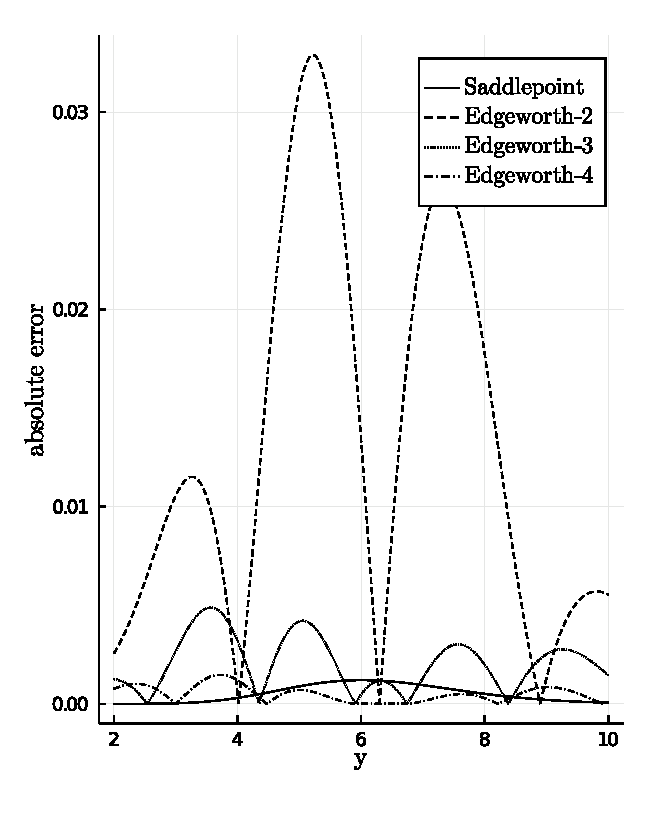
\includegraphics[width=8cm]{saddlepoint_and_edgeworth_err_abs_gamma21_10_terms.eps} 
    }
    \subfloat{
        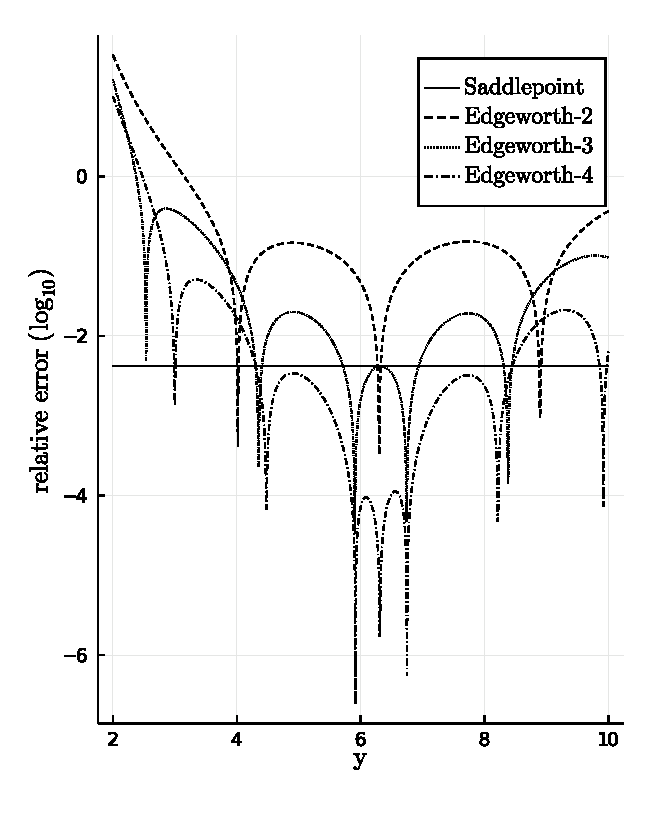
\includegraphics[width=8cm]{saddlepoint_and_edgeworth_err_rel_gamma21_10_terms.eps} 
    }
    \caption{Study of the approximation error of the Saddlepoint approximation on a standardized sum of $n=10$ of $\Gamma(2, 1)$ random variables. Both panel exposes properties studied of the Saddlepoint approximation: the accurate rellative error, the gain in order of approximation and the uniform relative error of the approximation for sums of Gamma random variables.}
    \label{fig-saddlepoint-err}
\end{figure}

\begin{example} \label{ex-gamma-saddle}
    Continuing Example \ref{ex-gamma-edge}, we can analyze the behaviour of the Saddlpoint approximation to the mean $Y = n^{-1}\sum_{i=1}^n X_i \in \R_+$ where $X_1, \ldots, X_n \simiid \Gamma(p, \lambda)$. The cumulant generating function of the $\Gamma(n, p)$ distribution is $K(t) = p\logf{\lambda} - p\logf{\lambda - t}$ and its first derivative is $K'(t) = p / (\lambda - t)$. For any $s \in \R_+$, the Saddlepoint $\hat\gamma_s$ is given by the solution to the Saddlepoint Equation (\ref{eq-saddlepoint}), which here becomes
    \begin{equation*}
        \frac{p}{\lambda - \hat\gamma_s/n} = s \Rightarrow \hat\gamma_s = n\left(\lambda - \frac{p}{s}\right).
    \end{equation*}
    In Figure \ref{fig-saddlepoint-err}, we demonstrate how the Saddlepoint approximation of order 3 compares to the Edgeworth apperoximation when approximating a standardized sum of $n$ random variables independently distributed acording to $\Gamma(2, 1)$. Since the standardized sum can be obtained by multiplying the mean by a factor of $\sqrt{n}$, the Saddlepoint approximation is easily adapted by change of variable. Both panels show accurate approximation properties both in terms of relative and absolute error.
    
    In this example, it is also interesting to examine the concrete form of the Saddlepoint approximation $g_3$. Replacing the relevant quantities in Equation (\ref{eq-saddle-3}), we obtain that the Saddlepoint approximation is
    \begin{align*}
        g_3(s; K) &= \sqrt{\frac{n}{2\pi K''(\lambda - \frac{p}{s})}} \expf{nK\left(\lambda - \frac{p}{s}\right) - n\left(\lambda - \frac{p}{s}\right)s}\\
        &= \sqrt{\frac{n}{2\pi s^2/p}} \expf{n\left(p\logf{\lambda} - p\logf{p/s}\right) - ns\lambda + np}\\
        &= (n\lambda)^{np}s^{np-1}\expf{-sn\lambda} \times \frac{(np)^{1/2-np}\expf{np}}{\sqrt{2\pi}}.
    \end{align*}
    Consider now the Stirling's formula for the gamma function
    \begin{equation*}
        \Gamma(z) = \sqrt{2\pi}z^{z-1/2}\expf{-z}(1 + O(z^{-1})).
    \end{equation*}
    We recognize that the second term in the expression of $g_3(s; K)$ corresponds to the inverse of the Stirling's approximation to $\Gamma(np)$. The Saddlepoint approximation to the density of the mean of $\Gamma(p, \lambda)$ variables thus corresponds to the density of the true distribution $\Gamma(np, n\lambda)$ of the mean, where the gamma function has been replaced by the Stirling's approximation. This has the interesting consequence that the relative error of the Saddlepoint approximation does not depend on $s$, the point at which the density is evaluated, but rather only depends on $n$. This behaviour is also exposed in Figure \ref{fig-saddlepoint-err} where the relative error of the Saddlepoint approximation is a straight horizontal line. Daniels \cite{daniels1954saddlepoint} characterizes the class of distributions for which the uniform relative approximation error holds.
\end{example}